\documentclass[sigconf]{acmart}
\usepackage{graphicx}
\usepackage{hyperref}
\usepackage{todonotes}

\usepackage{endfloat}
\renewcommand{\efloatseparator}{\mbox{}} % no new page between figures

\usepackage{booktabs} % For formal tables

\settopmatter{printacmref=false} % Removes citation information below abstract
\renewcommand\footnotetextcopyrightpermission[1]{} % removes footnote with conference information in first column
\pagestyle{plain} % removes running headers

\newcommand{\TODO}[1]{\todo[inline]{#1}}



\begin{document}

\title{TBI: A Data Driven Journey Beyond Contact Sports that  
Puts Data In The Driver's Seat}



\author{Jeffry L. Garner}
\affiliation{%
  \institution{Indiana University}
  \streetaddress{Online Student}
  \city{} 
  \state{} 
  \postcode{}
}
\email{jeffgarn@iu.edu}

\begin{abstract}

The data journey into concussions starts with the confluence of contact sports, long-term neurological diseases, and well known athletes.  Lots of fascinating technologies to help the hockey player, football player and others that play contact sports.  And hey, sports matter!  But the data journey leads down other roads.  The Data Scientist has an opportunity to help the athlete but also an opportunity to help many others as well.  This data journey is not well known and has far less panache but is important nonetheless.  This road leads to military veterans, those injured in auto-accidents, and the elderly.  We will take a deep dive into data from the Veterans Affairs department, and see what it tells us and what else can be done. 

\end{abstract}

\keywords{i523, hib315, Big Data, TBI, Veterans Affairs, Concussion}


\maketitle

\section{Introduction}

Be it a researcher, a developer, a scientist, a doctor, an accountant, a stay-at-home mom, or a DJ, we all want to know that we are making a difference.  For some, it's through one-time or episodic opportunities: service projects for some, for others it comes in the form of making a monetary donation, and for others, it's less formal: simply helping someone in person.  But for others, there is an opportunity to know that what they are doing day in and day out could help someone in a meaningful way.  It's particularly satisfying that what you may do for a living could indeed help someone in a consequential way.   For most of us we wonder if we are fulfilling that yearning within us.  The manager in the business that is trying to make a buck, or the employee at the license bureau, or the teaching assistant...those may have to seek out that extra bit of fulfillment or satisfaction.

Yes, indeed, we can all make a difference....even a Data Scientist!  Yes, in a small or large way a Data Scientist can make a real difference.  Ii it the keen Python skills that Data Scientists possess that make the difference?  Or is it the machine learning and R-programming that sets the data scientist apart?  Not likely, if not, then surely the ability to query a database, provide documentation, and manage a keen bibliography is the critical piece.  All of these are important to be clear.  However, a Data Scientist can make a true and meaningful difference by knowing and exercising two essential cornerstones of big data:  1) Knowing your data.  2) Being willing to take the road down which the data leads.  Sometimes its the journey that determines the destination.  Are you willing to go?


\section{The Beginning}

When the author was young, around 10 or 11 years old, he fell off his bike directly in front of his house.  He hit his head on the side of a cement sewer and received a concussion.  At the time, it was uncommon for a youth to wear a helmet.  The idea of wearing a helmet was not even thought about. He was not taken to the hospital or doctor for any treatment or diagnosis.  Therefore, there was nothing definitively diagnosed, medically speaking.   Nothing was quantitatively documented.  No X-Rays or MRI to test or verify. The only tangible {\em data} was a large knot on the side of his head, a loss of balance so bad that he could hardly walk or even stand upright, and tremendous nausea.  

Today there are concussion protocols.  At the slightest sign of concussion symptoms, the footballer is taken into a tent and examined by a physician.  We have learned the importance of a quick diagnosis and immediate treatment.  In today's professional game, we have means of measuring the g-force of each hit, using sensors within the helmet.  Wikipedia describes g-force (the ``g'' referencing gravity) as ``a measurement of the type of acceleration that causes a perception in weight.  Despite the name, it is incorrect to consider g-force a fundamental force, as ``g-force'' is a type of acceleration that can be measured with an accelerometer.  Since g-force accelerations indirectly produce weight, any g-force can be described as a `weight per unit mass'.  Helmet sensors can indicate the direction of the impact in addition to the g-force measurement.  This information is collected and real-time notifications are sent to trainers and even parents of young athletes.  

\section{Youth Athletics}

In recent years, due to health issues of high profile professional athletes, we are learning more about the long-term health impacts of head injuries sustained as a young adult or as a child.  Along with medical research, data has helped to pave the way for a growing understanding of the impacts of TBI (Traumatic Brain Injury) as well as impacts to the head that are not traumatic.  This is indeed critical as the incidents occur at a ''rate of 1.6-3.8 million in the United States per year with accumulated costs approaching \$60 billion annually.  Recent studies have identified relationships between magnitude, frequency and location of these sustained head impacts with post event symptoms and decrements in neurocognitive function.''\cite{www-theshockbox-com}

With mounting evidence that head impacts, as young adults, can impact our long-term neurological health, the previously quoted report from Shockbox research (one of several independent studies) drew still further concern.  It concludes, ``when monitored for head impacts across a regular season, it was seen that the elementary age players (average age of 13) experience a similar magnitude and frequency of impacts compared to the high school players (average age of 17).  The frequency and magnitude of high peak g impacts in elementary (71 impacts with 50 g average) causing 6 concussions is also similar to the high school team players (84 impacts with 51 g average) who did not have any team concussions.  It is also seen that youth players are still developing skills and techniques leading for increased impacts at the front of the head.'' \cite{www-theshockbox-com} 

While the ``data road'' is showing us information in terms of numbers, is the data diverse and comprehensive?  That is, we can measure force and impacts to the brain but what about other data sources like biological tests ({\em markers}) or images?  Patrick Bellgowan, a scientist at the University of Tulsa's Laureate Institute for Brain Research, focused his effort on measurement and {\em form} of the hippocampus.  The hippocampus is a major portion of the human brain and is part of the limbic system and thus plays a role in spacial memory, long and short-term memory, and is linked to processing and likely emotional control.  Bellgowan's research is published in the {\em Journal of the American Medical Association} and shows some very stark numbers. ``A group of 25 players with no history of reported concussions had hippocampuses that were, on average, 14 percent smaller than those of a control group of 25 males of similar age and health who didn't play contact sports.'' \cite{www-sportsonearth-com}  Further, the report shows that while ``much of the health and safety debate over football and other contact sports focuses on the risk of developing severe, headline-grabbing neurodegenerative diseases like amyotrophic lateral sclerosis (ALS) and CTE, a growing body of evidence suggests that both concussions and subconcussive blows can alter mood, cognition and behavior while causing damage and structural changes to the brain.'' \cite{www-sportsonearth-com}

Traveling down this ``data road'' there is no shortage of information around concussions, TBIs, and athletics.  We can certainly understand the concern with the potential long-term impacts on one's health.  Fear for our young athletes' health would concern any doctor, pediatrician and most certainly parents.  Based on the quantity of information one would think that it's the athlete that is most susceptible.  The youth are vulnerable to be sure, but is it only the athlete?  It's clear that professional athletics is big business in our country and around the world.  It wasn't until the deaths of the big name professional athletes that this issue came to the public's eye.  Researchers were already looking into this but focus was not sharpened until we heard the names of Mike Webster, Dave Duerson, Andre Waters and Junior Seau.  These athletes made millions and the big business of athletics was at stake.  With all this money comes more concern and interest and, in this case, data availability. 

However, this ``data road'' if you will, did not originate with athletics.  While the bulk of the data is based on TBI concerns for athletics, it originated with the military.  Military personnel have tremendous challenges with head trauma due to the force of explosions and projectiles.  With the military, the measured force of explosions and the speed of projectiles is tremendous especially when compared to the trauma experienced by most athletes.  Add to this, a soldier is under significant stress as part of his job.  How both head trauma along with significant levels of stress impacts the soldier's neurological health requires much more research, as do related TBIs in the general population due to auto accidents, falls and violence.  While culturally the impacts of TBIs on athletes garners greater attention, it's the military and the population at large that provides opportunities for the Data Scientist, if we let the data do the driving.  

\section{The General Population}

The Center for Disease Control and Prevention (CDC) is a great source for detailed information regarding TBI's and the general populous.  They are involved in providing detailed reports to congress and to the citizens regarding items related to our health.  While access to raw data is not available, the breadth and scope of the data that is available is worth studying.  The CDC provides data regarding the rates of hospital visits, emergency department visits, and death broken out by age group and type or cause of trauma.  Much of this data is available going back several years.  In addition, there are numerous reports including broad level statistics.  For example:

\begin{figure}[h]
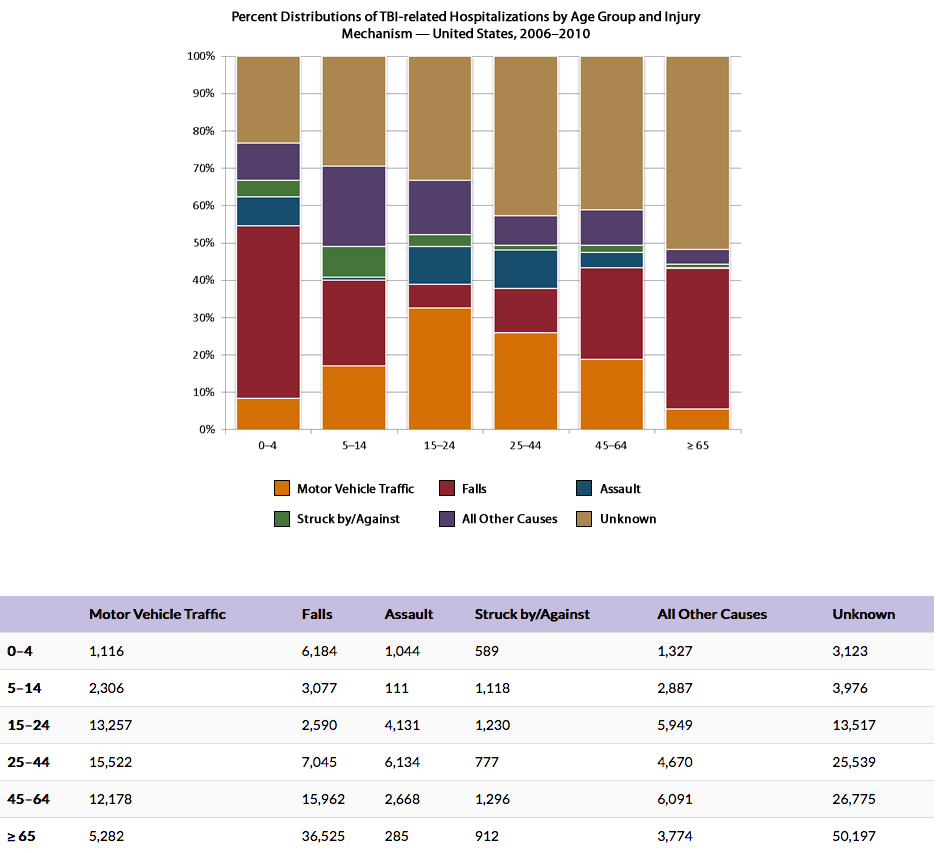
\includegraphics[width=\columnwidth]{images/graph1.png}
\caption{CDC TBI Type 2006-2010}\label{f:CDC TBI Type 2006-2010}
\end{figure}

It's by knowing the data that you can better understand the quality of the data.  If we want to make a difference, in data science, we have to know the source of the data.  The CDC leverages a few sources for their TBI related reporting.  The Healthcare Cost and Utilization Project (HCUP) is a part of the US Health and Human Services Department.  It's a comprehensive repository or collection of databases related to hospital stays and patient care data.  HCUP has yet another collection of databases called NEDS (Nationwide Emergency Department Sample) and NIS (National Impatient Sample).  The databases rely on data that is input and managed by hospitals at the time of the patients stay.  The CDC feels that the data ``sample size is large enough to provide stable annual estimates of TBI.''  

One way that these databases are created is due to the efforts at the hospital using the International Classification of Disease (ICD), in this case the ICD-9-CM, which is the {\em International Classification of Disease, Ninth Edition, Clinical Modification}.  To a Data Scientist this is a standardized basis of input of the source data - a very good thing.  During a patient's stay in the hospital, there is a standard in identifying the diagnosis as well as classifications, used for patient releases or secondary diagnoses.  For example, lets say a patient is admitted into the hospital with a TBI due to an auto accident in which the patient's head hits the steering wheel, causing injury. Code 804: multiple fractures involving skull or face with other bones, could be used.  Multiple codes could also be used to further define the extent of the injuries or diagnosis.  While this approach has inherit challenges for a data scientist, for example, how do we manage analysis tied to multiple codes, or potential administrative issues (loss of data or mis-classification)? The good thing is that we do have a standard and data that we can build upon.  And in this case, the data source has a standardization which is important. To help alleviate some of the aforementioned data concerns, we could minimize some of the data challenges by increasing the sample size or extrapolate by leveraging other similar sources to increase our certainty.

The CDC's published report ``Traumatic Brain Injury - Related Emergency Department Visits, Hospitalizations, and Deaths - United States, 2007 and 2013,'' concluded the following: ``In 2013, approximately 2.8 million TBI-related ED visits, hospitalizations, and deaths occurred in the United States, representing an increase in 2007 that was largely attributed to an increase in the number and rate of TBI - related ED (Emergency Departments), {\em i.e.}, Emergency Room visits.  Although much public interest has been devoted to sports-related concussion in youth, the findings in this report indicate that older adult falls account for a much larger proportion of the increase in TBI-related ED visits during this period.  In addition, although the modest increase in ED visits that might be attributed to youth sports concussions do not extend to increases in TBI-related hospitalizations and deaths, the same cannot be said for TBIs attributed to older adult falls.  From 2007 and 2013, increases in TBI-related hospitalizations and death attributable to older adult falls suggest the need for greater attention to preventing older adult falls.  Empirically validated prevention measures can help reduce the incidence of older adult falls.'' \cite{www-cdc-gov}.  By quantifying the causes of some of the TBI's for the general public, using data, we could indeed make a difference and help to ``empirically validate prevention measures''.

If the ICD codes were expanded to include more details around causation, or if during the hospital visit the symptoms were tagged to {\em potential} cause we could build upon that from a data perspective.  Knowing that some will not know the cause of the fall (elderly), or a patient could have been concussed due to domestic violence and is unwilling to discuss it, building upon what we currently have could help us use the data to help prevent TBIs in the general public.  The CDC created the STEADI program (Stopping Elderly Accidents, Deaths and Injuries), which is an effort to help identify older adults at risk and help prevent falls.  A Data Scientist research could marry results to those in the medical field for an opportunity to help with predictive analytics and preemptively provide support to the elderly and others at risk using the data we have and are building upon.  While there is so much attention paid to athletes and data tied to youth head injury prevention, there is a vast opportunity to help others, of all ages, and truly make a difference.  

\section{The Veterans}

On the playing field, athletes like to call it the ``Field of Battle''.  This analog represents the arena in which the athlete challenges himself to beat his opponent and win the game.  While the ''Field of Battle'' for the athlete offers a competitive challenge, it is not life or death.  The soldier, fights on THE field of battle.  He doesn't play to win but to live.  Balls are not flying but bullets!  This places an immeasurable amount of stress on the soldier.  Imagine adding a TBI to a critically stressed soldier.  The dynamics increase, and so does the need to understand the causes, health, history, and symptoms of the soldier.  In short, we need more data in order to help.

``While most people fully recover from a concussion within three to six months, soldiers who suffer concussions in battle can experience symptoms for years following the injury, says Michael K. Rauls, an experimental psychology student at Augusta State University in August.  Combat-related stress may prolong soldiers' recovery, and, at the same time, concussions may hamper solders' ability to recover from stress.''\cite{www-apa-org}

The following url provided raw data for examination.  This is data from the Veterans Affairs database accessible under the catalog of government data.  The data sets are available under the catalog section and is intended for public access and use.  In addition, Metadata has been created and was updated in November, 2017.  

url - https://catalog.data.gov/dataset/mild-tbi-diagnosis-and-management-strategies 
\cite{www-catalog-data-gov}

From the website, once you have accessed the catalog you will notice the source data used is JSON data via the website.  JSON (JavaScript Object Notation) is easy to access and is considered ``human-readable''.  We chose to convert the JSON to CSV (Common Separated Values) then uploaded via Python as well as input into excel. We converted CSV to XLSX, a Microsoft Excel format.  We analyzed the data for any obvious issues as this is normally a good time to do some data cleaning.  It's also a good time to do some realigning if need be, i.e., move some data around to align more cleanly.  At this point, we used the pivot function within excel.  The pivot function is one of excel's most powerful features.  It allows the user to align large data sets in order to extract meaning.  The result is a table like format that is easily used to make charts or graphs. 

Below is a snippet of the JSON data downloaded from the Veterans Affairs (VA) website.  


\begin{figure}[h]
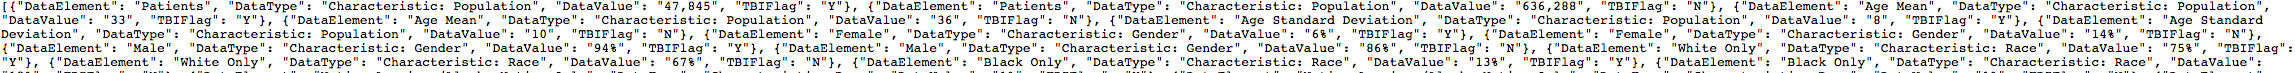
\includegraphics[width=\columnwidth]{images/graph2.png}
\caption{Veterans Affairs JSON}\label{f:Veterans Affairs JSON}
\end{figure}

Using a simple conversion tool, this image is a snippet of the JSON parsed data translated to CSV.

\begin{figure}[h]
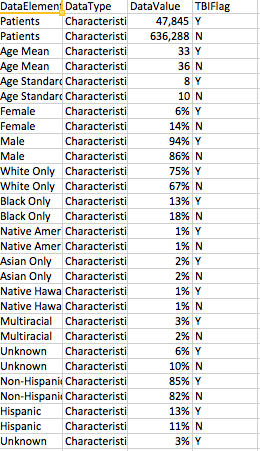
\includegraphics[width=\columnwidth]{images/graph3.png}
\caption{Veterans Affairs CSV}\label{f:Veterans Affairs CSV}
\end{figure}

Using Python, via Jupyter Notebook, to pull in the CSV for additional programming work.


\begin{figure}[h]
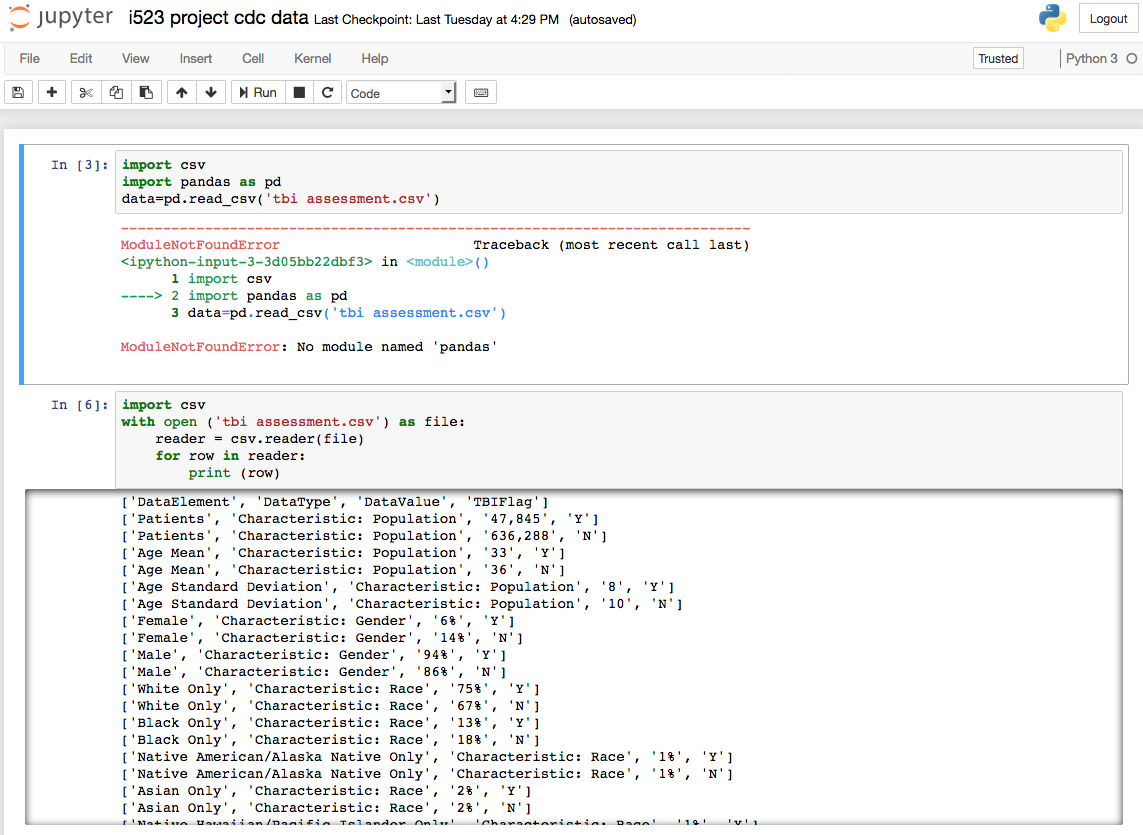
\includegraphics[width=\columnwidth]{images/graph4.png}
\caption{Veterans Affairs ipynb}\label{f:Veterans Affairs ipynb}
\end{figure}

There are two data sets: (1) Mild TBI Diagnosis and Management Strategies: Implications for Assessment and Treatment in Veterans (2) Mild TBI Diagnosis and Management Strategies: VA's TBI Screening and Evaluation Program. The Screening and Evaluation Program document contains primarily data, in terms of total numbers, related to the Veterans symptoms.  We will however dig deeper into the Assessment and Treatment in Veterans data.

This data from the Assessment and Treatment dataset is small and straightforward.  The data variables have four categories: DataElement, DataType, DataValue and TBIFlag.  TBIFlag is used to differentiate those that were diagnosed with TBI as the data set includes both those diagnosed with TBI and those that were not identified.  The working assumption is that there could be some that actually did have a Traumatic Brain Injury that may not have been officially diagnosed and flagged in this data. If you looked at it hierarchically, DataElement is the more granular of the two key characteristic variables.  So DataElement would be the ``child'' to the DataType, and is dependant on the DataType. 

The specific parsing and analyzing effort was to take the CSV file and import it into Microsoft Excel.  Using excel, for both datasets, we created a workbook in which to analyze the data, similar to a Jupyter Notebook used for Python.  We created a ``data tab'' which held the CSV data that we copied and placed into a pivot table.  Leveraging the two primary data variables of DataElement and DataType we analyzed the data.  Based on what the data told us we set up additional tabs as a work space in the workbook to look at particular DataTypes.  At this point, we created charts to illustrate the data findings, the most pertinent charts of which are included in this project.  This was done by the charting capabilities within excel.

The DataType includes several categories, but we will focus on a few.  One area was the ``category of care by patient with and without TBI''.  This data set included a total of 684,133 veterans that were patients.  Of that, 47,845 (7\%) had the TBI flag while the remaining 636,288 did not.  Included are some charts created from the data based on the {\em category of care} and as we expected, those with TBI (flagged for TBI) had a higher percentage of treatment related to Psychiatry and Mental Health.  

\begin{figure}[h]
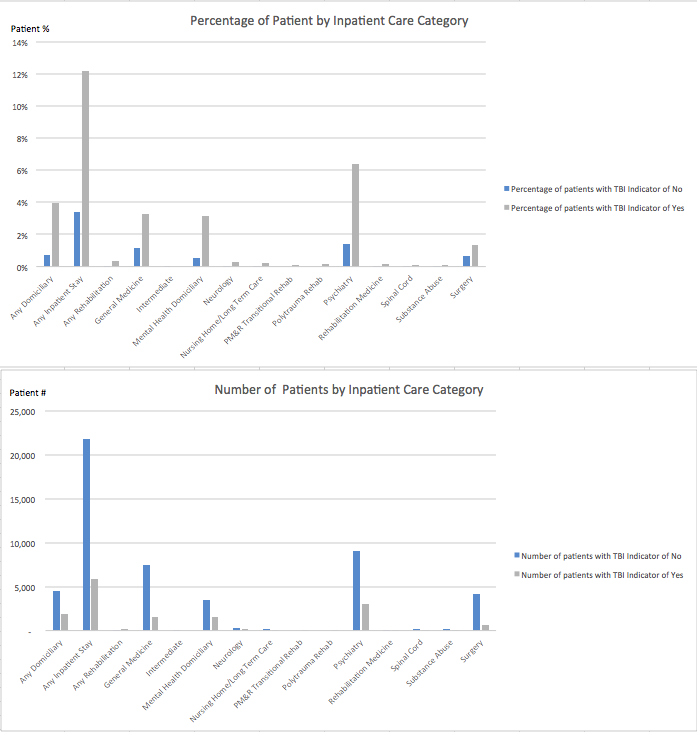
\includegraphics[width=\columnwidth]{images/graph5.png}
\caption{Veterans Affairs Care Category}\label{f:Veterans Affairs Care Category}
\end{figure}

Additionally, we looked into another DataType category of  ``Prevalence of Mental Health and Pain''.  This category includes DataValues of: depression, bipolar, psychosis, PTSD (Post-Traumatic Stress Disorder) and others.  While it was not clear, we are assuming this diagnosis of the prevalence of mental health and pain was made as a result of the treatment of TBI, though the data does include numbers on veterans who had been (prior to) receiving services from the VA (Veterans Affairs/Administration), listed as a ``VA User''.  The point here is there is some uncertainty as to whether their diagnoses were pre-TBI or were as a result of having a TBI.  The results, however, were particularly stark in that the veteran with TBI had a marked increase in areas around mental health, PTSD, headache and depression.   The chart shows the comparisons.

\begin{figure}[h]
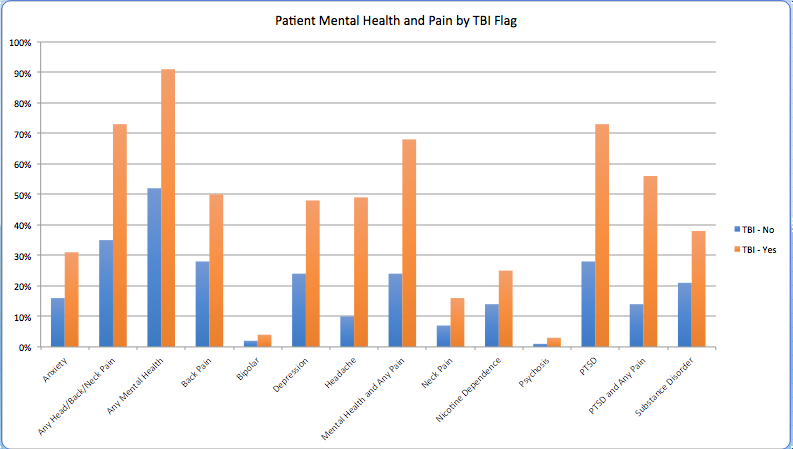
\includegraphics[width=\columnwidth]{images/graph6.png}
\caption{Veterans Affairs mental health and pain}\label{f:Veterans Affairs mental health and pain}
\end{figure}

One DataType that caught our eye was the ``Category of Care Inpatient Length of Stay'', since veterans with TBI and other stress related health issues should have a marked increase in the length of stay.  However, the TBI flagged veterans did not show an increase in the time of stay, the data did not represent a length of time.  Since time was not a DataElement option, we decided to compare the ``In-patient Stay'' percentages to the total number of patients and found that it was the result of the two.  Therefore, ``Category of Care Inpatient Length of Stay'', was not a representation of time but the number of patients.  The simple chart illustrates the result.  So {\em specifically} the length of stay is actually the ``Number of Patients by Inpatient Care Category'' shown in a prior chart. While we feel this is an error with the data, the general feeling is that we think it is minor but will reach out to the VA and advise.  However, it would have been interesting for this researcher to see that data.


\begin{figure}[h]
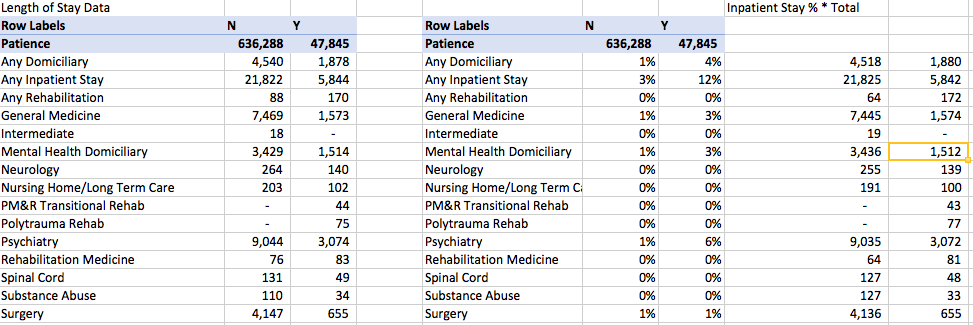
\includegraphics[width=\columnwidth]{images/graph7.png}
\caption{Veterans Affairs incorrect length of stay}\label{f:Veterans Affairs incorrect length of stay}
\end{figure}


While we do have errors in the data, the fact that the data does include Diagnosis Codes as a DataType variable is promising.  These are the same codes described prior as ICD (International Classification of Disease).  This helps to provide us with additional information that can be used to further help medical personnel and support of veterans who have prolonged rehabilitation due to TBIs and the various levels of stress, including PTSD.

The second of the two JSON data sets ``VA's TBI Screening and Evaluation Program'', includes yearly diagnosis numbers and ``Postconcussive Symptoms in the last 30 days.  The yearly diagnosis numbers at first blush appear to provide meaningful information as it includes a yearly total of patients as well as the percentage of those that were diagnosed with pain, or PTSD or TBI, which was very similar to the data in the first JSON data set.  Additionally, the overall year to year numbers should be reflective of the amount of military activity within that given year, assuming the concussions were directly related to military activity.  That is, I would expect to see the overall numbers, as well as those particular diagnosis numbers, increase when there is military activity.  This data does not provide any information regarding the level of activity by the military, within the given year.

However, the second JSON data set includes the ``Postconcussive Symptoms in the last 30 days'', which helps to support that data in the first JSON data set ``Implications for Assessment and Treatment''.  This data set evaluated 55,070 postconcussive veterans within 30 days.  My working assumption is that these veterans would have been diagnosed within the last 30 days, but could have sustained the concussion more than 30 days ago.  The postconcussive symptoms in this data set are numerous and center around the general categories of:  Anxiety, depression, fatigue, forgetfulness, headache, irritability among others.  For each symptom category the symptom is measured as either, none, mild or moderate to severe. 

The postconcussive symptoms that had the highest number of veterans, that was diagnosed with that symptom, all had moderate to severe measured symptoms.  The top five identified symptoms, all having a moderate to severe rating are: 1) Irritability (easily annoyed), 2) Sleep Disturbance, 3) Forgetfulness, 4) Anxious or tense and 5) Headaches.  For example, of the 55,070 postconcussive veterans, 45,389 felt irritable and were easily annoyed; which is 82 percent.  Over 72 percent complained of moderate to severe headaches.  It would be interesting to compare similar raw data from concussed athletes to these numbers to see how they compare.  


So what does all this data tell the Data Scientist?  The data driven direction has found that veterans and active soldiers with TBI are diagnosed at a higher rate in terms of levels of stress, and thus have a need for mental health treatment and psychiatric care.  As a result, recovery takes much longer than say the general population or for athletes and, based on the first JSON dataset, a majority of veterans were Veteran Affair or services users.  Given the data that we have, it appears that TBI veterans have as many symptoms and likely many more, and for a longer period of time, than athletes.  To that, veterans have the additional complication of stress that increases the symptoms and the severity.  Imagine a TBI veteran that is experiencing moderate to severe headaches, anxiety, fatigue and irritability.  Not only is the concern around the long-term neurological health, like Alzheimer's or CTE (Chronic Traumatic Encephalopathy), the veteran has to deal with a prolonged recovery {\em short-term}.  

How can the Data Scientist make a difference?  Given the data we have, we can start to create some models to help align the symptoms to care and start to leverage this based on each military mission.  In essence, prepare for the TBI patience, coming in from the battle field, regarding long-term care.  Since we have the ICD codes (diagnosis codes) in this data, can we use these or enhance the data to draw a connection to the causes of the TBI.  If so, by linking the causation, to the symptoms and recovery, we can prepare earlier, plan for the impact and the cost.  With the goal of ultimately working with the military to help limit TBIs.  The idea would be to use the information to help proactively identify soldiers at risk, diagnose quickly, and be prepared with the necessary treatment as quickly as possible, which includes planning for the future, as unlike the athlete who may need to quit playing a game, the solider may be giving up his job.  Anything the Data Scientist can do to help, would make a difference.


\section{The Challenges}

The desire of this research was to pull together a fascinating story to show that head trauma, even mild trauma, over a period of time could cause long-term debilitating neurological effects.  Furthermore, we wanted to show the benefit of documenting the daily head trauma of football players in both practice and games and then add all the data together and tell the story of how we now know that mild regular head trauma is just as dangerous as TBIs and maybe more so, as you may not know you are in long-term neurological danger.  This would have been supported by the output of helmet sensors and collection of data each and every day.  The daily data for each player would have been collected, cleaned and organized to show the direction of head impacts (what part of the brain was affected).  The data would have included a {\em g-force measurement} for each hit, again on a daily basis. 

All of the aforementioned would be linked to, and compared with, a regular MRI or another type of image.  Say for example, an annual MRI of the brain to compare year to year changes or to look for any changes due to the helmet impact data gathered throughout the year.  Any potential correlation from these two data sources would be documented.  From a data science perspective, we had envisioned a method to represent the images quantitatively so that we could more easily align the image to the daily impact data.  For example, we could divide the brain up alphabetically, each letter representing a different area within the brain.  To each alphabetically designated section, we could apply a combination of numeric value and a word, say a color, to illustrate both the location, type and severity of injury, or changes to the brain from the MRI.  For a Data Scientist then you can start to build some correlation between the daily data and the specific message in the image.  Gathered on an annual basis we could build some history and move towards doing some predictive-analytics.   To both the daily impact data and the images we could also include biological markers, that could be analyzed from blood to show concussions and other biological changes, further adding {\em richness} to the data.  However, we never found that data. Yes, medically speaking, some correlation or cause-and-effect data exist but not in an overall quantifiable manner and not available in a data set for the Data Scientist.

Finding medical data sets is a challenge to be sure.  We researched for days trying to find any data set with little luck.  We would expect that medical data sets would be limited due to privacy concerns and how quickly data in the medical world can become stale.  We would expect that some data sets were very challenging and expensive to gather and that the owner would not want to freely offer such an asset.  Then there is the likely challenge of the complexity of a given medical data set.  We would assume that most medical, in particular head trauma based, data sets would be complicated and challenging to access, parse, clean, read, etc.  However, it was a learning experience to find so little.  It also has us wondering if the medical community might be well served to have some other {\em eyes} looking at the data.  We read several medical studies and journals and know that there is indeed data available based on the research that was found, but nothing that was accessible.  As a result, this might be an excellent opportunity for data science, computer science and medical worlds to work together towards a shared goal, and make a difference.  This created a question for us that we were not able to have the time to further investigate.  

Since the data drove us to the general public and in particular head injuries to the military, we were not able to pull together information around the causes, other than high level information.  That is, by knowing more about the cause of the head trauma we may be able to better work toward limiting them.  We simply assumed one thing, but the data steered us in a different direction.  It would have been interesting to pursue any roll that big data could have played in helping to limit TBIs in the military.  Just the concussion from the delivery of a large artillery piece is significant.  Imagine being on the receiving end.

Not only was there limited data, but the JSON data sets were small.  The actual patient numbers were reasonable but the lack of historical data based on diagnosis types, or symptoms related to any long-term neurological diseases, or additional data on the patient recovery would have been welcomed.  Imagine then comparing this to a similar data set for athletes who had experienced TBI, which would have been very interesting.  It's from this point that we could build a cost-estimate related to treatment and recovery and then show the difference in cost for treatment of the athlete and the veteran.  For the Data Scientist, working towards pulling together a cost-estimate for veterans would help in preparing the necessary care as well as doing analysis on the benefits of prevention and additional research.  As for the veteran, their likely short-term treatment will take much longer than the athlete, not to mention the expense of the veteran not being able to work as well as any potential long-term impacts to the veteran, complexities not all athletes have to endure.  In theory, we might find that research dollars are better spent dealing with TBIs in veterans than the athlete.

Another challenge is trying to better understand what we don't know.   For example, the JSON data sets were based on those veterans receiving care from the VA.  We also know from the data that about 80\% of them had been receiving care from the VA prior, but we don't know how far back their VA based treatment and diagnosis went.  We also do not know how many soldiers were diagnosed on the battle field or training and are not receiving care from the VA and are therefore not identified in these numbers.  To the Data Scientist, it would be important to know of all the military personnel that were diagnosed with TBI, how many are in treatment with the VA?  

Lastly, as the paper outlines, we have a concern about the long-term effects of head trauma, especially repeated trauma.  Alzheimer's, CTE, Parkinson's diseases are catastrophic, and building an open relationship between these diseases and concussion are ongoing.  This is a growing area of research, as the medical research of the brain is complicated and still maturing.  Additionally, this type of research is a long-term endeavor as some of these diseases are not diagnosed until years after the head trauma.  So the challenge of gathering actionable data can take years - even decades.  Also, some of the disease identification requires research of the brain after the death of the patient.  It was not until after the doctors were able to examine the brains of athletes that they identified what is now called CTE.


\section{Conclusion}

``The road goes ever on and on, down from the door where it began.  Now far ahead the road has gone, and I must follow, if I can, pursuing it with eager feet, until it joins some larger way where many paths and errands meet.  And whither then?  I cannot say.'' - J.R.R. Tolkien, The Fellowship of the Ring.

The availability of data drove us down a different road than we expected.  It also opened our eyes to a brand new group affected by brain injuries - The Military!  While the data sets were limited, the research process placed us on a road that opened our eyes.  A road that was built upon not only concern of TBIs for athletes, but for the general population and the military.  

When compared to the athlete, the soldier needs so much more to recover.  The TBI's are worse, requiring a longer period of time to recover.  The extended recover time impacts life in the military and at home, thus impacting the quality of life as well as vocation, as they may be forced to retire or ultimately be disabled.  The potential long-term impacts are not insignificant.  Their road is one with hills.  We can't help but dream of what we can do to help.

With more data, we can make a difference in identifying the injured.  With more data we can build towards complete rehabilitation and treatment.  And with more data we can help prepare for the financial challenges.  With all the resources and companies lined up to help the athlete, as well as substantial financial resources from sports leagues and institutions...we wonder if our veterans will be treated similarly.  Will we maintain the quality of helmet sensors for our soldier that the star football player receives?  Will we keep a database and track impacts to our soldiers like Riddell helmet company does for the high school football player?  If not, the data may just show us what we are not doing for our veterans.  That is a road worth traveling one that is making a difference....welcome to Data Science. 




\begin{acks}

Many thanks to Professor Gregor von Laszewski, the Teaching Assistants and Indiana University.  I also want to thank Katie, my understanding wife.  Lastly, for my employer AT\&T for a commitment to education and giving me 26 years of experience, challenge and opportunity.

\end{acks}



\bibliographystyle{ACM-Reference-Format}
\bibliography{report} 

\end{document}


